\begin{name}
	{\tenchude}
	{\tendethi}
	{\tentruong}
	{\thoigian}
	\end{name}
\TN
\Opensolutionfile{ans}[ans/de1-phanI]
\begin{ex}%Câu 1
	Cho cấp số nhân $(u_n)$ với $u_1=2$ và $u_4=16$. Công bội của cấp số nhân đã cho bằng
	\choice
	{$q=4$}
	{\True $q=2$}
	{$q=-2$}
	{$q=-4$}
	\loigiai{
		Ta có $\dfrac{u_4}{u_1}=\dfrac{16}{2}=8=q^3$ nên $q=2$.}
\end{ex}
\begin{ex}%Câu 2
	Cho khối lăng trụ đứng có cạnh bên bằng $5$, đáy là hình vuông có cạnh bằng $4$. Hỏi thể tích của khối lăng trụ bằng bao nhiêu?
	\choice
	{$100$}
	{$20$}
	{$64$}
	{\True $80$}
	\loigiai{
		Ta có thể tích khối lăng trụ bằng $4^2\cdot 5=80$.}
\end{ex}
\textbf{\textit{Sử dụng thông tin dưới đây để trả lời câu \ref{câu 3-đề 1} và câu \ref{câu 4-đề 1}}}\\[0.5em]
Cho hàm số đa thức bậc ba $y=f(x)$ có bảng biến thiên như hình vẽ dưới đây
\begin{center}
	
\begin{tikzpicture}
		\tkzTabInit[nocadre=false,lgt=1.2,espcl=2.5,deltacl=0.6]
		{$x$ /0.6, $y'$ /0.6, $y$ /2}
		{$-\infty$,$-1$,$1$,$+\infty$}
		\tkzTabLine{,+,$0$,-,$0$,+,}
		\tkzTabVar{-/$-\infty$,+/$2$,-/$-2$,+/$+\infty$}
	\end{tikzpicture}
\end{center}
\begin{ex}%Câu 3
	\label{câu 3-đề 1}
	Giá trị cực đại của hàm số $y=f(x)$ bằng
	\choice
	{$y_{\text{CĐ}}=-2$}
	{\True $y_{\text{CĐ}}=2$}
	{$y_{\text{CĐ}}=-1$}
	{$y_{\text{CĐ}}=1$}
	\loigiai{
		Dựa vào bảng biến thiên, ta có $y_{\text{CĐ}}=2$.}
\end{ex}
\begin{ex}%Câu 4
	\label{câu 4-đề 1}
	Hàm số nào dưới đây có bảng biến thiên như hình vẽ trên?\vspace{3pt}
	\choice
	{$y=\dfrac{x+1}{x-1}$}
	{$y=-x^3+3x$}
	{$y=x^3+3x$}
	{\True $y=x^3-3x$}
	\loigiai{
		Hàm số có bảng biến thiên như trên có tập xác định là $\mathbb{R}$, đạo hàm có hai nghiệm là $x=1$ và $x=-1$ nên ta loại phương án $\circled{A}$ và $\circled{C}$.\\
		Lại có, $f(x)$ tiến về $+\infty$ khi $x\to+\infty$ nên ta chọn đáp án $\circled{D}$.}
\end{ex}
\begin{ex}%Câu 5
	Tập nghiệm của bất phương trình $3^{-x}\ge\dfrac{1}{27}$ là
	\choice
	{$(-\infty;-3)$}
	{$[3;+\infty)$}
	{$[-3;+\infty)$}
	{\True $(-\infty;3]$}
	\loigiai{
		Ta có $3^{-x}\geq\dfrac{1}{27}\Leftrightarrow -x\geq\log_3\left(\dfrac{1}{27}\right)=-3\Leftrightarrow x\leq 3$.}
\end{ex}
\begin{ex}%Câu 6
	Trong không gian $Oxyz$, cho mặt cầu $(S)\colon x^2+y^2+z^2-4x+2y-2z-3=0$. Tìm tọa độ tâm $I$ và bán kính $R$ của $(S)$.
	\choice
	{\True $I(2;-1;1)$ và $R=3$}
	{$I(-2;1;-1)$ và $R=3$}
	{$I(2;-1;1)$ và $R=9$}
	{$I(-2;1;-1)$ và $R=9$}
	\loigiai{
		Ta có $x^2+y^2+z^2-4x+2y-2z-3=0\Leftrightarrow (x-2)^2+(y+1)^2+(z-1)^2=9$.\\
		Do đó, tâm $I(2;-1;1)$ và $R=3$.}
\end{ex}
\begin{ex}%Câu 7
	Mệnh đề nào \textbf{sai} trong các mệnh đề sau?\vspace{3pt}
	\choice[0.5em]
	{$\displaystyle\int \dfrac{1}{\sin^2 x} \mathrm{\,d}x=-\cot x+C$}
	{$\displaystyle\int \cos x \mathrm{\,d}x=\sin x+C$}
	{$\displaystyle\int \dfrac{1}{\cos^2 x} \mathrm{\,d}x=\tan x+C$}
	{\True $\displaystyle\int \sin x \mathrm{\,d}x=\cos x+C$}
	\loigiai{
		Ta có $\displaystyle\int \sin x \mathrm{\,d}x=-\cos x+C$.}
\end{ex}
\begin{ex}%Câu 8
	Với $a$ là số thực dương tùy ý, $\log_{\sqrt{3}}\left(9a^3\right)$ bằng\vspace{3pt}
	\choice
	{\True $4+6\log_3 a$}
	{$1+\dfrac{3}{2}\log_3 a$}
	{$4-6\log_3 a$}
	{$1-\dfrac{3}{2}\log_3 a$}
	\loigiai{
		Ta có $\log_{\sqrt{3}}\left(9a^3\right)=2\cdot\log_3\left(9a^3\right)=2\cdot\left(2+3\log_3 a\right)=4+6\log_3 a$.}
\end{ex}
\renewcommand{\baselinestretch}{1.55}
\begin{ex}%Câu 9
	\immini[thm]
	{
		Cho hình chóp $S.ABCD$ có đáy là hình bình hành (như hình vẽ minh họa). Hãy chọn khẳng định đúng trong các khẳng định sau.\vspace{3pt}
		\choice[0.3em]
		{\True $\overrightarrow{SA}+\overrightarrow{SC}=\overrightarrow{SB}+\overrightarrow{SD}$}
		{$\overrightarrow{SA}+\overrightarrow{AB}=\overrightarrow{SD}+\overrightarrow{DC}$}
		{$\overrightarrow{SA}+\overrightarrow{AD}=\overrightarrow{SB}+\overrightarrow{BC}$}
		{$\overrightarrow{SA}+\overrightarrow{SB}=\overrightarrow{SC}+\overrightarrow{SD}$}
	}
	{
		\begin{tikzpicture}[scale=0.6,>=stealth, font=\footnotesize, line join=round, line cap=round]
			\def\a{4}
			\path 	(0:0) coordinate (A)
			++(0:\a) coordinate (D)
			++(-130:\a/2) coordinate (C)
			($(A)+(C)-(D)$) coordinate (B)
			($(A)+(80:\a)$) coordinate (S)
			(intersection of A--C and B--D) coordinate (O);%giao điểm O
			\draw[dashed,thick] 	(B)--(A)--(D)	(A)--(S);
			\draw[thick] 			(B)-- (C)--(D)
			(B)--(S)	(C)--(S)	(D)--(S);
			\foreach \x/\g in {A/135,B/-135,C/-45,D/45,S/90}
			\fill[black] 	(\x) circle (1pt)
			($(\g:3mm)+(\x)$) node {$\x$};	
		\end{tikzpicture}
	}
	\loigiai{
		Ta có $\overrightarrow{SA}+\overrightarrow{SC}=\overrightarrow{SB}+\overrightarrow{SD}\Leftrightarrow \overrightarrow{SA}-\overrightarrow{SB}=\overrightarrow{SD}-\overrightarrow{SC}\Leftrightarrow \overrightarrow{BA}=\overrightarrow{CD}$.\\
		Do $ABCD$ là hình bình hành nên $\overrightarrow{BA}=\overrightarrow{CD}$ là đẳng thức đúng.}
\end{ex}
\vspace{15pt}
\begin{ex}%Câu 10
	\immini[thm]
	{
		Hình thang cong $ABCD$ ở hình vẽ bên có diện tích bằng\vspace{3pt}
		\choice[0.3em]
		{$\displaystyle\int\limits_{1}^{3} \left(\dfrac{3}{x}-x+2\right) \mathrm{\,d}x$}
		{$\displaystyle\int\limits_{1}^{3} \left(\dfrac{3}{x}-x-2\right) \mathrm{\,d}x$}
		{$\displaystyle\int\limits_{1}^{3} \left(\dfrac{3}{x}+x+2\right) \mathrm{\,d}x$}
		{\True $\displaystyle\int\limits_{1}^{3} \left(\dfrac{3}{x}+x-2\right) \mathrm{\,d}x$}
	}
	{
		\begin{tikzpicture}[scale=0.6,>=stealth, font=\footnotesize, line join=round, line cap=round]
			\def\xmin{-1} \def\xmax{4}
			\def\ymin{-2} \def\ymax{4} 
			\draw[->] (\xmin,0)--(\xmax,0) node [below]{$x$};
			\draw[->] (0,\ymin)--(0,\ymax) node [left]{$y$};
			\node at (0,0) [below left]{$O$};
			\draw (3,-1.8)node[]{$y=-x+2$} (1,4.2)node[]{$y=\dfrac{3}{x}$};
			\clip (\xmin+0.1,\ymin+0.1) rectangle (\xmax-0.5,\ymax-0.1);
			\draw[smooth,samples=300,domain=\xmin:\xmax] plot(\x,{-(\x)+2});
			\draw[smooth,samples=300,domain=0.1:\xmax] plot(\x,{3/(\x)});
			\draw[dashed] (1,0)node[below]{$1$}--(1,3)--(0,3)node[left]{$3$} (0,-1)node[left]{$-1$}--(3,-1)--(3,0)node[below right]{$3$}--(3,1)--(0,1)node[left]{$1$};
			\fill (1,1)node[below left]{$A$}circle(1pt);
			\fill (1,3)node[above right]{$B$}circle(1pt);
			\fill (3,1)node[above right]{$C$}circle(1pt);
			\fill (3,-1)node[below]{$D$}circle(1pt);
			\fill[color=gray,opacity=0.4] plot[domain=1:3](\x,{3/(\x)})--plot[domain=3:1](\x,{-(\x)+2})--cycle;
		\end{tikzpicture}
	}
	\loigiai{
		Hình thang cong bị giới hạn bởi các đường  $y=\dfrac{3}{x}$, $y=-x+2$, $x=1$ và $x=3$.\\
		Trong khoảng $(1;3)$ đồ thị hàm số $y=\dfrac{3}{x}$ nằm trên đồ thị hàm số $y=-x+2$ nên diện tích hình thang cong $ABCD$ bằng $\displaystyle\int\limits_{1}^{3} \left(\dfrac{3}{x}+x-2\right) \mathrm{\,d}x$.}
\end{ex}
\begin{ex}%Câu 11
	Trong không gian $Oxyz$, cho mặt phẳng $(P)\colon 2x-y-2z+3=0$. Đường thẳng $\Delta$ đi qua điểm $M(4;1;-3)$ và vuông góc với $(P)$ có phương trình chính tắc là\vspace{4pt}
	\choice[0.3em]
	{$\dfrac{x+4}{2}=\dfrac{y+1}{-1}=\dfrac{z-3}{-2}$}
	{$\dfrac{x-2}{4}=\dfrac{y+1}{1}=\dfrac{z+2}{-3}$}
	{$\dfrac{x+2}{2}=\dfrac{y+2}{1}=\dfrac{z-3}{-2}$}
	{\True $\dfrac{x-4}{2}=\dfrac{y-1}{-1}=\dfrac{z+3}{-2}$}
	\loigiai{
		Đường thẳng $\Delta$ vuông góc với $(P)$ nên có một vectơ chỉ phương là $(2;-1;-2)$.\\
		Phương trình chính tắc của $\Delta$ là $\dfrac{x-4}{2}=\dfrac{y-1}{-1}=\dfrac{z+3}{-2}$.}
\end{ex}
\begin{ex}%Câu 12
	Kết quả khảo sát năng suất (đơn vị: tấn/ha) của một số thửa ruộng được minh họa ở biểu đồ sau
	\begin{center}
		\begin{tikzpicture}[line join=round, line cap=round,>=stealth,xscale=1.2,yscale=0.7,font=\footnotesize,scale=0.8]
			\def\a{1}
			\def\xmax{9}
			\def\ymax{7}
			\tikzset{label style/.style={font=\footnotesize}}
			\draw[->] (0,0)--(\xmax,0) node[below] {\text{Năng suất (tấn/ha)}};
			\draw[->] (0,0)--(0,\ymax) node[left] {\text{Số thửa ruộng}};
			\draw (0,0) node [below left] {$O$};
			\draw[thin]
			(0,1)--(\xmax,1)
			(0,2)--(\xmax,2)
			(0,3)--(\xmax,3)
			(0,4)--(\xmax,4)
			(0,5)--(\xmax,5)
			(0,6)--(\xmax,6)
			;
			\foreach \i in {1,2,3,4,5,6}{
				\draw (0,\i) node[left]{$\i$};
			}
			%		\foreach \i/\j in {0.5*\a/3,1.5*\a/4,2.5*\a/6,3.5*\a/5,4.5*\a/5,5.5*\a/2}{
				%			\draw (\i,\j) node[above]{$\j$};
				%		}
			\foreach \i/\j in {1.5*\a/{$[5{,}5;5{,}7)$},2.5*\a/{$[5{,}7;5{,}9)$},3.5*\a/{$[5{,}9;6{,}1)$},4.5*\a/{$[6{,}1;6{,}3)$},5.5*\a/{$[6{,}3;6{,}5)$},6.5*\a/{$[6{,}5;6{,}7)$}}{
				\draw (\i-0.1,-0.6) node[below,rotate=45]{$\j$};
			}
			\fill[blue!20]
			(\a,0) rectangle (2*\a,3)
			(2*\a,0) rectangle (3*\a,4)
			(3*\a,0) rectangle (4*\a,6)
			(4*\a,0) rectangle (5*\a,5)
			(5*\a,0) rectangle (6*\a,5)
			(6*\a,0) rectangle (7*\a,2)
			;
			\begin{scope}
				\draw
				(\a,3)--(2*\a,3) 
				(2*\a,4)--(3*\a,4)
				(3*\a,6)--(4*\a,6)
				(4*\a,5)--(5*\a,5)
				(5*\a,5)--(6*\a,5)
				(6*\a,2)--(7*\a,2)
				(\a,0)--(\a,3)
				(2*\a,0)--(2*\a,4)
				(3*\a,0)--(3*\a,6)
				(4*\a,0)--(4*\a,6)
				(5*\a,0)--(5*\a,5)
				(6*\a,0)--(6*\a,5)
				(7*\a,0)--(7*\a,2)
				;
				\draw (3.5,\ymax) node[above]{\textbf{Năng suất lúa của một số thửa ruộng}};
			\end{scope}
		\end{tikzpicture}
	\end{center}
	Lập bảng tần số ghép nhóm ta tính được khoảng tứ phân vị của mẫu số liệu trên \textbf{gần bằng} giá trị nào dưới đây?
	\choice
	{$0{,}3$}
	{$0{,}4$}
	{\True $0{,}5$}
	{$0{,}6$}
	\loigiai{
		Bảng tần số ghép nhóm của mẫu số liệu trên.
		\begin{center}
			\begin{tabular}{|c|c|c|c|c|c|c|}
				\hline
				Nhóm &$[5{,}5;5{,}7]$ &$[5{,}7;5{,}9]$  &$[5{,}9;6{,}1]$  &$[6{,}1;6{,}3]$  &$[6{,}3;6{,}5]$  &$[6{,}5;6{,}7]$  \\
				\hline
				Tần số &$3$ &$4$  &$6$  &$5$  &$5$  &$2$  \\
				\hline
			\end{tabular}
		\end{center}
		Mẫu số liệu có $25$ giá trị nên trung vị là giá trị thứ $13$.\\ 
		Do đó, tứ phân vị thứ nhất là trung bình cộng của giá trị thứ $6$ và thứ $7$ nên $Q_1\in[5{,}7;5{,}9]$, tứ phân vị thứ ba là trung bình cộng của giá trị thứ $19$ và $20$ nên $Q_3\in[6{,}3;6{,}5]$.\\
		Ta có $Q_1=5{,}7+\dfrac{\dfrac{25}{4}-3}{4}\cdot0{,}2=5{,}8625$; $Q_3=6{,}3+\dfrac{\dfrac{25\cdot 3}{4}-18}{5}\cdot0{,}2=6{,}33$.\\
		Vậy khoảng tứ phân vị $\Delta_Q=6{,}33-5{,}8625=0{,}4675\approx 0{,}5$.}
\end{ex}
\Closesolutionfile{ans}
%\renewcommand{\baselinestretch}{1.35}
%{\fontfamily{qtm}\fontsize{13pt}{2pt}\selectfont\textbf{PHẦN II. Câu trắc nghiệm đúng sai}. Thí sinh trả lời từ câu 1 đến câu 4. Trong mỗi ý \textbf{a)}, \textbf{b)}, \textbf{c)}, \textbf{d)} ở mỗi câu, thí sinh chọn đúng hoặc sai.}
%\setcounter{ex}{0}% Reset lại số đếm câu hỏi
\TNTF
\Opensolutionfile{ans}[ans/de1-phanII]
\begin{ex}%Câu 1
	Cho hàm số $f(x)=\left(x^2-3x-3\right)\mathrm{e}^x$. Xét tính đúng sai của các mệnh đề sau
	\choiceTF
	{\True Hàm số đã cho xác định với mọi $x\in\mathbb{R}$}
	{Đạo hàm của hàm số đã cho là $f'(x)=\left(x^2+x-6\right)\mathrm{e}^x$}
	{\True Phương trình $f'(x)=0$ có hai nghiệm thực phân biệt}
	{\True Hàm số $f(x)$ nghịch biến trên khoảng $(-2;3)$}
	\loigiai{
		\begin{itemchoice}
			\itemch \textbf{Đúng.}\\
			Hàm số đã cho là tích của hàm đa thức và hàm mũ nên tập xác định là $\mathbb{R}$.
			\itemch \textbf{Sai.}\\
			Ta có $f'(x)=(2x-3)\cdot\mathrm{e}^x+(x^2-3x-3)\cdot\mathrm{e}^x=(x^2-x-6)\mathrm{e}^x$.
			\itemch \textbf{Đúng.}\\
			Ta có $f'(x)=0\Leftrightarrow (x^2-x-6)\mathrm{e}^x=0\Leftrightarrow x^2-x-6=0\Leftrightarrow\hoac{&x=-2 \\&x=3.}$
			\itemch \textbf{Đúng.}\\
			Ta có $f'(x)\leq 0\Leftrightarrow (x^2-x-6)\mathrm{e}^x\leq 0\Leftrightarrow x^2-x-6\leq 0\Leftrightarrow -2\leq x\leq 3$.\\
			Vậy hàm số nghịch biến trên $[-2;3]$ nên cũng nghịch biến trên $(-2;3)$.
	\end{itemchoice}}
\end{ex}
\begin{ex}%Câu 2
	Một nắp bể nước hình chữ nhật $ABCD$ nằm cạnh bờ tường có kích thước $9\text{ dm}\times 12\text{ dm}$ được kéo ra từ mặt sàn, do tác dụng của trọng lực nên nắp bể không thể mở ra được nếu không có người giữ. Người ta dùng một sợi dây dài $15$ dm và kéo căng nối đỉnh $C$ của hình chữ nhật với điểm $M$ nằm phía trên bờ tường sao cho $AM=9$ dm và $AM$ vuông góc với mặt sàn. Chọn hệ trục $Oxyz$ như hình vẽ, khi đó nắp bể mở ra và tạo với mặt sàn một góc $\alpha$ (đơn vị trên mỗi trục tọa độ tính bằng dm). Bỏ qua độ dày của nắp bể.
	\immini{
	Xét tính đúng sai của các mệnh đề sau
	\choiceTF
	{Điểm $M$ thuộc mặt phẳng có phương trình $z=0$}
	{Tọa độ điểm $C$ là $C\left(9\sin\alpha;12;9\cos\alpha\right)$}
	{Góc giữa nắp bể và mặt sàn sau khi kéo lên là $\alpha=60^\circ$}
	{\True Phương trình mặt phẳng chứa nắp bể sau khi kéo lên là $x-\sqrt{3}z=0$}}
	{\begin{tikzpicture}[scale=0.5,>=stealth, font=\footnotesize, line join=round, line cap=round]
			\draw[fill=gray!90] (-6.4,1.5)--(-6,1.3)--(-5.82,-3.49)--(-2.02,-6.02)--(5.8,-1.33)--(6.2,-1.6)--(-2,-6.52)--(-6.2,-3.72)--cycle;
			\draw[fill=gray!40] (-6.4,1.5)--(1.1,5.7)--(1.4,5.44)--(-6,1.3)--cycle;
			\draw[fill=gray!60] (-6,1.3)--(1.4,5.44)--(2,1.2)--(-5.82,-3.49)--cycle;
			\draw (1.4,5.44)--(2,1.2)--(6.2,-1.6);
			\coordinate (A) at (0,0);
			\coordinate (C) at (-1.42,-2.71);
			\coordinate (D) at (-4.3,-2.58);
			\coordinate (B) at ($(A)+(C)-(D)$);
			\draw[fill=black!60,opacity=0.9] (A)--(B)--(C)--(D)--cycle;
			\draw[fill=black!80] (B)--(3.05,-0.28)--(-1.42,-2.97)--(-3.99,-2.85)--(-4.3,-2.58)--(-1.42,-2.71)--cycle;
			\coordinate (E) at (-1.73,-4.82);
			\coordinate (F) at ($(A)+(E)-(D)$);
			\coordinate (M) at (0,3.72);
			\draw (D)--(E) (A)--(F) (E)--(F) (M)node[above right]{$M$}--(C);
			\fill[gray!40] (-5.82,-3.49)--(-2.02,-6.02)--(5.8,-1.33)--(2,1.2)--(A)--(B)--(3.05,-0.28)--(1.44,-1.25)--(F)--(E)--(D)--cycle;
			\draw[->] (0,0)node[above left,xshift=0.1cm,yshift=-0.1cm]{$O$}--(0,6)node[right]{$z$};
			\draw[->] (2,1.2)--(-7,-4.2)node[above]{$y$};
			\draw[->] (0,0)--(5.9,-3.5)node[above]{$x$};
			\draw (A)node[above right,yshift=0.2cm,xshift=-0.1cm]{$A$} (B)node[above]{$B$} ($(A)!0.5!(B)$)node[above,xshift=0.1cm]{$9$ dm} ($(A)!0.5!(D)$)node[above,xshift=-0.25cm]{$12$ dm} (D)node[above]{$D$} (C)node[above left]{$C$} (D)node[xshift=0.7cm,yshift=-0.4cm]{$\alpha$};
			\draw[dashed] (C) to[bend left] (E);
			\draw[dashed] (B) to[bend left] (F);
			\draw[decorate,decoration={markings,mark=between positions 2mm and \pgfdecoratedpathlength-2mm step 2mm with{\draw[black] (-3.5mm,-1.25mm) to[out=0,in=160] (-2mm,-1.25mm) to[out=-20,in=160] (2mm,1.25mm) to[out=-20,in=180] (3.5mm,1.25mm);}}] (M) -- (C);
			\fill (A)circle(3pt);
			\fill (B)circle(3pt);
			\fill (C)circle(3pt);
			\fill (D)circle(3pt);
			\fill (M)circle(3pt);
	\end{tikzpicture}}
	\loigiai{
		\begin{itemchoice}
			\itemch \textbf{Sai.}\\
			Điểm $M\in (Oxz)$ có phương trình $x=0$.
			\itemch \textbf{Sai.}\\
			Tọa độ điểm $C$ là $C(9\cos\alpha;12;9\sin\alpha)$.
			\itemch \textbf{Sai.}\\
			Ta có 
			\begin{align*}
				CM=15\Leftrightarrow CM^2=225&\Leftrightarrow (9\cos\alpha)^2+12^2+(9\sin\alpha-9)^2=225\\
				&\Leftrightarrow 81+12^2+9^2-162\sin\alpha=225\\
				&\Leftrightarrow162\sin\alpha=81\\
				&\Leftrightarrow\sin\alpha=\dfrac{1}{2}\Leftrightarrow\alpha=30^\circ.
			\end{align*}
			\itemch \textbf{Đúng.}\\
			Mặt phẳng chứa nắp bể sau khi kéo lên đi qua $3$ điểm $A(0;0;0)$, $C\left(\dfrac{9\sqrt{3}}{2};12;\dfrac{9}{2}\right)$ và $D(0;12;0)$.\\
			Do đó, vectơ pháp tuyến của mặt phẳng cùng phương với $\left[\overrightarrow{AC},\overrightarrow{AD}\right]$.\\
			Ta có $\overrightarrow{AC}=\left(\dfrac{9\sqrt{3}}{2};12;\dfrac{9}{2}\right)$, $\overrightarrow{AD}=(0;12;0)$ nên $\left[\overrightarrow{AC},\overrightarrow{AD}\right]=(-54;0;54\sqrt{3})$.\\
			Suy ra một vectơ pháp tuyến của mặt phẳng là $\overrightarrow{n}=(1;0;-\sqrt{3})$.\\
			Vậy phương trình mặt phẳng là $x-\sqrt{3}z=0$.
	\end{itemchoice}}
\end{ex}
\begin{ex}%Câu 3
	Trong một ngôi làng có $500$ người thì $240$ người là nam. Thống kê cho thấy rằng, khả năng mắc bệnh hô hấp ở người nam trong làng là $0{,}6\%$ và ở người nữ trong làng là $0{,}35\%$. Giả sử gặp một người trong làng.
	\begin{itemize}
		\item Gọi $A$ là biến cố \lq\lq gặp người mắc bệnh trong làng\rq\rq.
		\item Gọi $B$ là biến cố \lq\lq gặp được nam trong làng\rq\rq.
	\end{itemize}
	Xét tính đúng sai của các mệnh đề sau\vspace{3pt}
	\choiceTF
	{\True $\mathrm{P}(\overline{B})=\dfrac{13}{25}$}
	{Xác suất có điều kiện $\mathrm{P}(A\mid\overline{B})=0{,}006$}
	{Tỉ lệ mắc bệnh hô hấp chung của cả làng là $0{,}42\%$}
	{Giả sử có một người trong làng không mắc bệnh. Xác suất để người đó là nữ bằng $47{,}94\%$}
	\loigiai{
		\begin{itemchoice}
			\itemch \textbf{Đúng.}\\
			Ta có $\mathrm{P}(B)=\dfrac{240}{500}=\dfrac{12}{25}\Rightarrow\mathrm{P}(\overline{B})=1-\dfrac{12}{25}=\dfrac{13}{25}$.
			\itemch \textbf{Sai.}\\
			Ta có $\mathrm{P}(A\mid\overline{B})=0{,}35\%=0{,}0035$.
			\itemch \textbf{Sai.}\\
			Ta có $\mathrm{P}(A)=\mathrm{P}(B)\cdot\mathrm{P}(A\mid B)+\mathrm{P}(\overline{B})\cdot\mathrm{P}(A\mid\overline{B})=\dfrac{12}{25}\cdot 0{,}6\%+\dfrac{13}{25}\cdot 0{,}35\%=0{,}47\%$.
			\itemch \textbf{Sai.}\\
			Ta cần tính $\mathrm{P}(\overline{B}\mid \overline{A})$. Ta có $\mathrm{P}(\overline{B}\mid \overline{A})=\dfrac{\mathrm{P}(\overline{B})\cdot\mathrm{P}(\overline{A}\mid\overline{B})}{\mathrm{P}(\overline{B})\cdot\mathrm{P}(\overline{A}\mid\overline{B})+\mathrm{P}(B)\cdot\mathrm{P}(\overline{A}\mid B)}$.\\
			Lại có $\mathrm{P}(\overline{A}\mid\overline{B})=99{,}65\%$, $\mathrm{P}(\overline{A}\mid B)=99{,}4\%$. Do đó, $\mathrm{P}(\overline{B}\mid\overline{A})=\dfrac{\dfrac{13}{25}\cdot99{,}65\%}{\dfrac{13}{25}\cdot99{,}65\%+\dfrac{12}{25}\cdot 99{,}4\%}\approx 52{,}06\%$.
	\end{itemchoice}}
\end{ex}
\renewcommand{\baselinestretch}{1.55}
\begin{ex}%Câu 4
	Một quần thể vi khuẩn $(A)$ có số lượng cá thể là $P(t)$ sau $t$ phút quan sát được phát hiện thay đổi với tốc độ là $P'(t)=a\mathrm{e}^{0{,}1t}+150\mathrm{e}^{-0{,}03t}$ (vi khuẩn/phút) $(a\in\mathbb{R})$. Biết rằng lúc bắt đầu quan sát, quần thể có $200\,000$ vi khuẩn và đạt tốc độ tăng trưởng là $350$ vi khuẩn/phút. Xét tính đúng sai của các mệnh đề sau
	\choiceTF
	{\True Giá trị của $a=200$}
	{$P(t)=2\,000\mathrm{e}^{0{,}1t}-5\,000\mathrm{e}^{-0{,}03t}+200\,000$}
	{\True Sau $12$ phút số lượng vi khuẩn trong quần thể là $206\,152$ con (làm tròn kết quả đến hàng đơn vị)}
	{Sau $12$ phút, một quần thể vi khuẩn $(B)$ có tốc độ tăng trưởng là $G'(t)=500\mathrm{e}^{0{,}2t}$ (vi khuẩn/phút) bắt đầu cạnh tranh nguồn thức ăn trực tiếp với quần thể $(A)$, một cá thể tại quần thể $(B)$ triệt tiêu một cá thể tại quần thể $(A)$. Sau $5$ phút cạnh tranh quần thể $(A)$ bị triệt tiêu hoàn toàn. Số lượng vi khuẩn của quần thể $(B)$ ở thời điểm bắt đầu cạnh tranh là $191\,967$ con (làm tròn kết quả đến hàng đơn vị)}
	\loigiai{
		\begin{itemchoice}
			\itemch \textbf{Đúng.}\\
			Tại $t=0$, ta có $P'(0)=350\Leftrightarrow a+150 =350\Leftrightarrow a=200$.
			\itemch \textbf{Sai.}\\
			Ta có 
			\begin{align*}
				P(t)=\displaystyle\int P'(t)\mathrm{\,d}t&=\int\left(200\mathrm{e}^{0{,}1t}+150\mathrm{e}^{-0{,}03t}\right)\mathrm{\,d}t\\
				&=\dfrac{200}{0{,}1}\mathrm{e}^{0{,}1t} - \dfrac{150}{0{,}03}\mathrm{e}^{-0{,}03t}+C\\
				&=2\,000\mathrm{e}^{0{,}1t} - 5\,000\mathrm{e}^{-0{,}03t}+C.
			\end{align*}
			Tại $t=0$, ta có $P(0)=200\,000\Leftrightarrow 2\,000-5\,000+ C= 200\,000\Leftrightarrow C=203\,000$.\\
			Vậy $P(t)=2\,000\mathrm{e}^{0{,}1t}-5\,000\mathrm{e}^{-0{,}03t}+203\,000$.
			\itemch \textbf{Đúng.}\\
			Ta có $P(12)=2\,000\mathrm{e}^{0{,}1\cdot12}-5\,000\mathrm{e}^{-0{,}03\cdot 12}+203\,000\approx 206\,152$.
			\itemch \textbf{Sai.}\\
			Sau $5$ phút từ khi quần thể $(B)$ xuất hiện, số lượng vi khuẩn của quần thể $(A)$ là $P(17)\approx 210\, 945$ con.\\
			Ta có số lượng vi khuẩn của quần thể $(B)$ là $G(t)=\displaystyle\int G'(t)\mathrm{\,d}t=2\,500\mathrm{e}^{0{,}2t}+C$.\\
			Vì một cá thể tại quần thể $(B)$ triệt tiêu một cá thể tại quần thể $(A)$ và sau $5$ phút cạnh tranh quần thể $(A)$ bị triệt tiêu hoàn toàn nên $G(5)=P(17)$, tức là
			\[2\,500\mathrm{e}^{0{,}2\cdot5}+C=210\, 945\Leftrightarrow C\approx 204\, 149.\]
			Vậy số lượng vi khuẩn của quần thể $(B)$ ban đầu là $G(0)\approx 206\,649$ vi khuẩn.
	\end{itemchoice}}
\end{ex}
\Closesolutionfile{ans}
%{\fontfamily{qtm}\fontsize{13pt}{2pt}\selectfont\textbf{PHẦN III. Câu trắc nghiệm trả lời ngắn}. Thí sinh trả lời từ câu 1 đến câu 6 và điền đáp án vào ô trống.}
%\setcounter{ex}{0}% Reset lại số đếm câu hỏi
\TNSA
\Opensolutionfile{ans}[ans/de1-phanIII]
\begin{ex}%Câu 1
	% \immini[thm]
	% {
		Cho hình lập phương $ABCD.A'B'C'D'$ có cạnh $a$. Gọi $I$ là trung điểm của cạnh $BD$. Góc giữa hai đường thẳng $A'D$ và $B'I$ bằng bao nhiêu độ?
	% }
	% {
	% 	\begin{tikzpicture}[scale=0.75,>=stealth, font=\footnotesize, line join=round, line cap=round]
	% 		\def\a{3.5}
	% 		\path 	(0:0) coordinate (A)
	% 		++(0:\a) coordinate (D)
	% 		++(-130:\a/2) coordinate (C)
	% 		($(A)+(C)-(D)$) coordinate (B)
	% 		($(A)+(90:\a)$) coordinate (A')
	% 		($(B)+(90:\a)$) coordinate (B')
	% 		($(C)+(90:\a)$) coordinate (C')
	% 		($(D)+(90:\a)$) coordinate (D')
	% 		($(B)!0.5!(D)$) coordinate (I)
	% 		;
	% 		\draw[dashed,thick] 	(B)--(A)--(D)	(A)--(A');
	% 		\draw[thick] 	(C)--(C') 	(D)--(D') 	(B)--(B') 	(B)--(C)--(D) (A')--(B')--(C')--(D')--cycle;
	% 		\foreach \x/\g in {A/180,B/180,C/0,D/0,A'/180,B'/180,C'/0,D'/0}
	% 		\fill[black] 	(\x) circle (1pt)
	% 		($(\g:4mm)+(\x)$) node {$\x$};	
	% 	\end{tikzpicture}
	% }
	\shortans[0]{$30$}
	\loigiai{
		\begin{center}
			\begin{tikzpicture}[scale=0.75,>=stealth, font=\footnotesize, line join=round, line cap=round]
				\def\a{3.5}
				\path 	(0:0) coordinate (A)
				++(0:\a) coordinate (D)
				++(-130:\a/2) coordinate (C)
				($(A)+(C)-(D)$) coordinate (B)
				($(A)+(90:\a)$) coordinate (A')
				($(B)+(90:\a)$) coordinate (B')
				($(C)+(90:\a)$) coordinate (C')
				($(D)+(90:\a)$) coordinate (D')
				($(B)!0.5!(D)$) coordinate (I)
				;
				\draw[dashed,thick] 	(B)--(A)--(D)	(A)--(A') (B)--(D)--(A') (B')--(I);
				\draw[thick] 	(C)--(C') 	(D)--(D') 	(B)--(B')--(C) 	(B)--(C)--(D) (A')--(B')--(C')--(D')--cycle;
				\foreach \x/\g in {A/180,B/180,C/0,D/0,A'/180,B'/180,C'/0,D'/0,I/-90}
				\fill[black] 	(\x) circle (1pt)
				($(\g:4mm)+(\x)$) node {$\x$};	
			\end{tikzpicture}
		\end{center}
		Ta có $A'D\parallel B'C$ nên $(A'D,B'I)=(B'C,B'I)=\widehat{IB'C}$.\\
		Lại có $B'C=a\sqrt{2}$, $IC=\dfrac{a\sqrt{2}}{2}$, $B'I=\sqrt{BI^2+BB'^2}=\sqrt{\dfrac{a^2}{2}+a^2}=\dfrac{a\sqrt{6}}{2}$.\\
		Do đó, $\cos\widehat{IB'C}=\dfrac{B'C^2+B'I^2-IC^2}{2B'I\cdot B'C}=\dfrac{\sqrt{3}}{2}\Rightarrow\widehat{IB'C}=30^\circ$.}
\end{ex}
\vspace{15pt}
\begin{ex}%Câu 2
	\immini[thm]
	{
		Từ kho $D$ xe bưu chính đến lấy thư từ các hộp thư tại $E$, $F$, $G$ và $H$ rồi quay lại kho. Sơ đồ bên hiển thị thời gian xe bưu chính di chuyển giữa các hộp thư (đơn vị: phút). Thời gian ngắn nhất để xe bưu chính thực hiện điều đó là bao nhiêu phút?
	}
	{
		\begin{tikzpicture}[scale=0.81,>=stealth, font=\footnotesize, line join=round, line cap=round]
			\coordinate (H) at (0,0);
			\coordinate (G) at (4,0);
			\coordinate (E) at (2.5,4);
			\coordinate (D) at (-0.5,2);
			\coordinate (F) at (4.6,2.4);
			\draw (E)--(D)--(H)--(G)--(F)--cycle (E)--(H) (E)--(G) (D)--(F) (D)--(G) (H)--(F);
			\foreach \x/\g in {D/180,E/90,F/0,G/-45,H/-150} 
			\fill[black] (\x) circle(2pt) +(\g:4mm) node {$\x$};
			\draw ($(E)!0.5!(D)$)node[above left]{$11$} ($(E)!0.5!(F)$)node[above right]{$7$} ($(D)!0.5!(H)$)node[below left]{$3$} ($(G)!0.5!(F)$)node[below right]{$13$} ($(H)!0.6!(F)$)node[above left,yshift=-0.15cm]{$10$} ($(D)!0.6!(F)$)node[above]{$9$} ($(E)!0.7!(G)$)node[right]{$10$} ($(D)!0.4!(G)$)node[above]{$7$} ($(H)!0.7!(E)$)node[left]{$9$} ($(H)!0.5!(G)$)node[below]{$6$};
		\end{tikzpicture}
	}
	\shortans[0]{$35$}
	\loigiai{
		Xét một lộ trình di chuyển thỏa đề bài, chẳng hạn $D\to E\to F\to G\to H\to D$. Ta nhận thấy trong lộ trình di chuyển này, tại mỗi điểm, xe bưu chính bao giờ cũng sẽ có một tuyến đường vào và có một tuyến đường ra. Chẳng hạn, tại $D$ tuyến đường vào là $H\to D$, tuyến đường ra là $D\to E$.\\
		Điều này cho ta thấy, để chọn một lộ trình thỏa mãn đề bài, ta phải bỏ đi $2$ trong $4$ tuyến đường xuất phát từ mỗi đỉnh của sơ đồ.\\
		Mặt khác, sơ đồ có tất cả $10$ tuyến đường và một lộ trình thỏa mãn chỉ cần $5$ tuyến nên số đường đi phải bỏ đi là $5$.
		Để thời gian di chuyển của xe bưu chính là ngắn nhất thì tổng thời gian trên $5$ tuyến bị bỏ đi phải là lâu nhất. Tuyến đường nhiều thời gian nhất thỏa mãn lập luận trên là $D\to E\to H\to F\to G\to D$, thời gian thực hiện là $50$.\\
		Mà tổng thời gian trên các tuyến đường là $85$ nên thời gian ngắn nhất để xe bưu chính thực hiện là $85-50=35$ phút.}
\end{ex}
\vspace{15pt}
\begin{ex}%Câu 3
	\immini[thm]
	{
		Kiến trúc sư thiết kế một khu sinh hoạt cộng đồng có dạng hình vuông $ABCD$ có độ dài đường chéo $AC=120$ m. Trong đó, phần được tô màu đậm là sân chơi, phần còn lại để trồng hoa. Mỗi phần trồng hoa có đường biên cong là một phần của đường parabol với đỉnh thuộc một trục đối xứng của hình vuông, khoảng cách từ đỉnh đó đến đỉnh tương ứng của hình vuông bằng $40$ m và\break $AM=MN=NB$ (xem hình minh họa). Diện tích của phần sân chơi là bao nhiêu mét vuông? (làm tròn kết quả đến hàng đơn vị).
	}
	{
		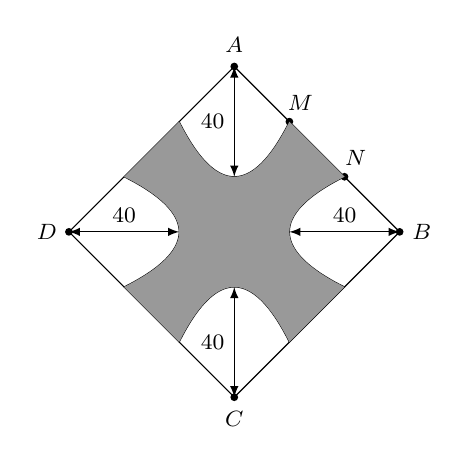
\begin{tikzpicture}[scale=0.7,>=stealth, font=\footnotesize, line join=round, line cap=round]
			\coordinate (A) at (0,3);
			\coordinate (B) at (3,0);
			\coordinate (C) at (0,-3);
			\coordinate (D) at (-3,0);
			\coordinate (M) at (1,2);
			\coordinate (N) at (2,1);
			\draw (A)--(B)--(C)--(D)--cycle;
			\draw[smooth,samples=300,domain=-1:1] plot(\x,{(\x)^2+1});
			\draw[smooth,samples=300,domain=-1:1] plot(\x,{-(\x)^2-1});
			\draw[smooth,samples=300,domain=-1:1] plot({(\x)^2+1},{\x});
			\draw[smooth,samples=300,domain=-1:1] plot({-(\x)^2-1},{\x});
			\foreach \x/\g in {A/90,B/0,C/-90,D/180,M/60,N/60} 
			\fill[black] (\x) circle(2pt) +(\g:4mm) node {$\x$};
			\draw[latex-latex] (A)--(0,1);
			\draw[latex-latex] (B)--(1,0);
			\draw[latex-latex] (C)--(0,-1);
			\draw[latex-latex] (D)--(-1,0);
			\draw (0,2)node[left]{$40$} (0,-2)node[left]{$40$} (2,0)node[above]{$40$} (-2,0)node[above]{$40$};
			\fill[color=gray!80] plot[domain=-1:1](\x,{(\x)^2+1})--plot[domain=1:-1]({(\x)^2+1},{\x})--plot[domain=1:-1](\x,{-(\x)^2-1})--plot[domain=-1:1]({-(\x)^2-1},{\x})--cycle;
		\end{tikzpicture}
	}
	\shortans[0]{$3467$}
	\loigiai{
		\begin{center}
			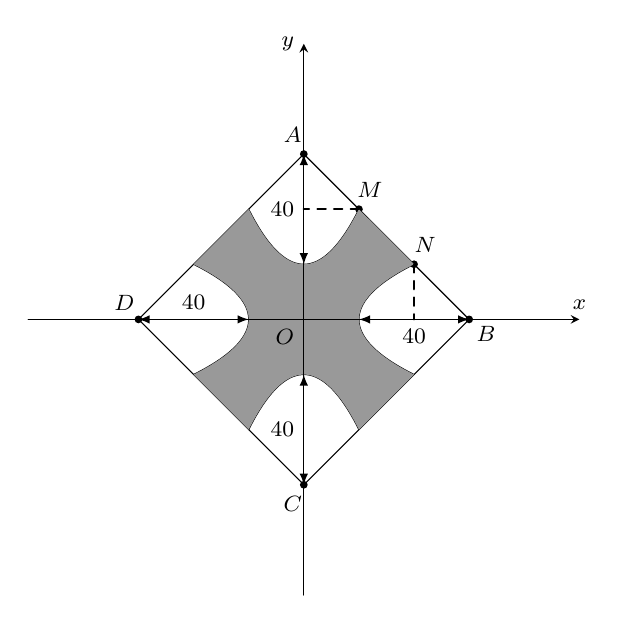
\begin{tikzpicture}[scale=0.7,>=stealth, font=\footnotesize, line join=round, line cap=round]
				\coordinate (A) at (0,3);
				\coordinate (B) at (3,0);
				\coordinate (C) at (0,-3);
				\coordinate (D) at (-3,0);
				\coordinate (M) at (1,2);
				\coordinate (N) at (2,1);
				\draw (A)--(B)--(C)--(D)--cycle;
				\draw[smooth,samples=300,domain=-1:1] plot(\x,{(\x)^2+1});
				\draw[smooth,samples=300,domain=-1:1] plot(\x,{-(\x)^2-1});
				\draw[smooth,samples=300,domain=-1:1] plot({(\x)^2+1},{\x});
				\draw[smooth,samples=300,domain=-1:1] plot({-(\x)^2-1},{\x});
				\foreach \x/\g in {A/120,B/-40,C/-120,D/130,M/60,N/60} 
				\fill[black] (\x) circle(2pt) +(\g:4mm) node {$\x$};
				\draw[latex-latex] (A)--(0,1);
				\draw[latex-latex] (B)--(1,0);
				\draw[latex-latex] (C)--(0,-1);
				\draw[latex-latex] (D)--(-1,0);
				\draw (0,2)node[left]{$40$} (0,-2)node[left]{$40$} (2,0)node[below]{$40$} (-2,0)node[above]{$40$};
				\fill[color=gray!80] plot[domain=-1:1](\x,{(\x)^2+1})--plot[domain=1:-1]({(\x)^2+1},{\x})--plot[domain=1:-1](\x,{-(\x)^2-1})--plot[domain=-1:1]({-(\x)^2-1},{\x})--cycle;
				\path 	(0,0) coordinate (O);	
				\draw[-stealth] (-5,0)--(5,0)node[above]{$x$};
				\draw[-stealth] (0,-5)--(0,5)node[left]{$y$};
				\node [below left] at (0,0) {$O$};
				\draw[dashed, thick] (2,1)--(2,0) (1,2)--(0,2); 
			\end{tikzpicture}
		\end{center}
		Ta chọn hệ trục tọa độ $Oxy$ như hình vẽ, trong đó $O$ là giao điểm hai đường chéo $AC$ và $BD$, trục $Ox$ trùng với đường thẳng $BD$, trục $Oy$ trùng với đường thẳng $AC$.\\
		Khi đó, tọa độ các điểm là $A(0;60)$, $B(60;0)$, $C(0;-60)$, $D(-60;0)$.\\
		Vì $AM=MN=NB$ nên $\overrightarrow{AM}=\dfrac{1}{3}\overrightarrow{AB}$. Giả sử $M(x;y)$, khi đó $\heva{&x=\dfrac{1}{3}\cdot 60=20 \\&y-60=\dfrac{1}{3}\cdot(-60)=-20}\Leftrightarrow\heva{&x=20 \\&y=40.}$\\
		Tương tự, ta có $\overrightarrow{AN}=\dfrac{2}{3}\overrightarrow{AB}$ nên $N(40;20)$.\\
		Đường parabol đi qua điểm $M$ có đỉnh nằm trên trục $Oy$, cắt trục $Oy$ tại điểm có tung độ $20$ có phương trình là $y=\dfrac{1}{20}x^2+20$.\\
		Đường parabol đi qua điểm $N$ có đỉnh nằm trên trục $Ox$, cắt trục $Ox$ tại điểm có hoành độ $20$ có phương trình là $x=\dfrac{1}{20}y^2+20$.\\
		Ta gọi $(H_1)$ là hình giới hạn bởi parabol $y=\dfrac{1}{20}x^2+20$, trục $Oy$, đường thẳng $AM$ có phương trình $y=-x+60$.\\
		Ta gọi $(H_2)$ là hình giới hạn bởi parabol $x=\dfrac{1}{20}y^2+20$, trục $Ox$, đường thẳng $BN$ có phương trình $y=-x+60$.\\
		Khi đó, \[S_{H_1}=\displaystyle\int\limits_{20}^{40}\sqrt{20\cdot(y-20)}\mathrm{\,d}y+\int\limits_{40}^{60}(60-y)\mathrm{\,d}y=\dfrac{1\,400}{3};\quad S_{H_2}=\displaystyle\int\limits_{20}^{40}\sqrt{20\cdot(x-20)}\mathrm{\,d}x+\int\limits_{40}^{60}(60-x)\mathrm{\,d}x=\dfrac{1\,400}{3}.\]
		Vậy diện tích một phần tư sân chơi bẳng $S_{AOB}-S_{H_1}-S_{H_2}=\dfrac{1}{2}\cdot 60\cdot 60 -2\cdot\dfrac{1\,400}{3}=\dfrac{2\,600}{3}$ nên diện tích sân chơi là $4\cdot\dfrac{2\,600}{3}\approx 3\,467$ m$^2$.}
\end{ex}
\renewcommand{\baselinestretch}{1.5}
\begin{ex}%Câu 4
	Sách Toán của một đơn vị xuất bản được in tại hai phân xưởng $A$ và $B$ và được vận chuyển về kho sau khi in xong. Xưởng $A$ có nhiệm vụ in $60\%$ tổng số lượng sách, xưởng $B$ sẽ in số lượng sách còn lại. Biết rằng số lượng sách Toán xưởng $A$ và $B$ in đạt yêu cầu về chất lượng và chuyển về kho lần lượt là $95\%$ và $90\%$. Nhân viên kiểm kho chọn ra ngẫu nhiên một cuốn sách Toán để kiểm tra thì thấy cuốn sách này không đạt yêu cầu về chất lượng. Xác suất để cuốn sách Toán đó được in ở xưởng $A$ là bao nhiêu phần trăm? (Làm tròn kết quả đến hàng phần chục).
	
	\shortans[0]{$42{,}9$}
	\loigiai{
		Gọi $M$ là biến cố quyển sách được in ở xưởng $A$, $N$ là biến cố quyển sách in không đạt yêu cầu về chất lượng.\\
		Theo đề, ta cần tính $\mathrm{P}(M\mid N)=\dfrac{\mathrm{P}(M)\cdot\mathrm{P}(N\mid M)}{\mathrm{P}(M)\cdot\mathrm{P}(N\mid M)+\mathrm{P}(\overline{M})\cdot\mathrm{P}(N\mid \overline{M})}$.\\
		Lại có $\mathrm{P}(M)=0{,}6$, $\mathrm{P}(\overline{M})=0{,}4$, $\mathrm{P}(N\mid M)=0{,}05$, $\mathrm{P}(N\mid \overline{M})=0{,}1$.\\
		Suy ra $\mathrm{P}(M\mid N)\approx 42{,}9\%$.}
\end{ex}
\begin{ex}%Câu 5
	\immini[thm]{Một phần của đường chạy của tàu lượn siêu tốc khi gắn hệ trục tọa độ $Oxy$ được mô phỏng ở hình dưới. Biết đường chạy của nó có dạng đồ thị hàm số bậc ba $y=ax^3+bx^2+cx+d$ $(0\le x\le 90)$; tàu lượn xuất phát từ điểm $A$ đồng thời đi qua các điểm $B$, $C$, $D$ (như hình vẽ). Đơn vị mỗi trục là mét, dựa vào đồ thị hình dưới, em hãy tính độ cao lớn nhất (theo đơn vị mét) mà tàu lượn siêu tốc đạt được so với mặt đất (xem $Ox$ là mặt đất). Kết quả làm tròn đến hàng phần mười.}
	{\begin{tikzpicture}[scale=0.7,>=stealth, font=\footnotesize, line join=round, line cap=round]
			\def\a{-1/15} \def\b{13/15} \def\c{-8/3} \def\d{3} % Hệ số
			\def\xmin{-1} \def\xmax{10}
			\def\ymin{-1} \def\ymax{5} 
			\draw[->] (\xmin,0)--(\xmax,0) node [below]{$x$};
			\draw[->] (0,\ymin)--(0,\ymax) node [left]{$y$};
			\node at (0,0) [below left]{$O$};
			\clip (\xmin+0.1,\ymin+0.1) rectangle (\xmax-0.5,\ymax-0.1);
			\draw[smooth,samples=300,domain=0:9] plot(\x,{\a*(\x)^3+\b*(\x)^2+\c*(\x)+\d});
			\draw[dashed] (3,0)node[below]{$30$}--(3,1)node[above]{$B$}--(0,1)node[left]{$10$} (5,0)node[below]{$50$}--(5,3)node[above]{$C$} (8,0)node[below]{$80$}--(8,3)node[above right]{$D$} (0,3)node[left]{$30$} (0,3)node[above right]{$A$}--(8,3);
	\end{tikzpicture}}	
	\shortans[0]{$39{,}9$}
	\loigiai{
		Đồ thị hàm số bậc ba đi qua điểm $A(0;30)$ nên $d=30$. Lại có, đồ thị đi qua điểm $B(30;10)$, $C(50;30)$, $D(80;30)$ nên ta có hệ phương trình sau
		\[\heva{&a\cdot 30^3+b\cdot 30^2+c\cdot30 +30=10 \\&a\cdot 50^3+b\cdot 50^2+c\cdot50 +30=30 \\&a\cdot 80^3+b\cdot 80^2+c\cdot80 +30=30}\Leftrightarrow\heva{&a=-\dfrac{1}{1\,500} \\&b=\dfrac{13}{150} \\&c=-\dfrac{8}{3}.}\]
		Ta có $f(x)=-\dfrac{1}{1\,500}x^3+\dfrac{13}{150}x^2-\dfrac{8}{3}x+30$. Khi đó, $f'(x)=-\dfrac{1}{500}x^2+\dfrac{13}{75}x-\dfrac{8}{3}$.\\
		Phương trình $f'(x)=0\Leftrightarrow -\dfrac{1}{500}x^2+\dfrac{13}{75}x-\dfrac{8}{3}=0\Leftrightarrow\hoac{&x=20 \\&x=\dfrac{200}{3}.}$\\
		Dựa vào đồ thị, ta thấy tàu đạt độ cao lớn nhất so với mặt đất khi đi qua điểm cực đại của đồ thị hàm số $f(x)$. Độ cao lớn nhất khi đó bằng $f\left(\dfrac{200}{3}\right)\approx 39{,}9$ m.}
\end{ex}
\begin{ex}%Câu 6
	\immini[thm]{Một quả bóng hình cầu có bán kính $r$ đang được treo trong một góc tường nhà (hai bờ tường vuông góc), một điểm $B$ cố định nằm trên mép của hai bờ tường và cách mặt đất $80$ cm, sợi dây treo bóng có độ dài $AB=30$ cm và đây cũng là độ dài ngắn nhất nối điểm $B$ với mặt xung quanh của quả bóng.\\
	Biết rằng quả bóng tiếp xúc với hai bên bờ tường và điểm thấp nhất của quả bóng cách mặt đáy $20$ cm. Hỏi đường kính của quả bóng là bao nhiêu centimet (làm tròn kết quả đến hàng đơn vị).
	}
	{\begin{tikzpicture}[scale=1,>=stealth, font=\footnotesize, line join=round, line cap=round]
			\fill[gray!60] (0,0)--(-1.8,-0.52)--(-1.8,3.98)--(0,4.5)--cycle;
			\fill[gray!35] (-1.8,-0.52)--(-2.69,0)--(-2.69,4.5)--(-1.8,3.98)--cycle;
			\fill[gray!35] (0,0)--(0,4.5)--(1.45,3.65)--(1.45,-0.85)--cycle;
			\fill[gray!60] (1.45,-0.85)--(2.36,-0.58)--(2.36,3.92)--(1.45,3.65)--cycle;
			\coordinate (I) at (-0.16,1.58);
			\coordinate (B) at (0,4);
			\coordinate (r) at (-0.69,1.03);
			\coordinate (x) at (-0.16,-0.52);
			\coordinate (L) at (0.29,-0.52);
			%			\tkzInterLC[R](I,B)(I,1.06)\tkzGetPoints{D}{A}
			%			\tkzInterLC[R](I,x)(I,1.06)\tkzGetPoints{E}{F}
			\draw[shading=ball,ball color=gray,opacity=0.8,name path=C1] (I) circle(1.06cm);
			\path[name path=IB] (I)--(B);
			\path[name path=Ix] (I)--(x);
			\path  	[name intersections={of=C1 and IB,by={A}}];	
			\path  	[name intersections={of=C1 and Ix,by={D}}];	
			\fill (I)circle(1.5pt);
			\fill (B)circle(1.5pt);
			\draw[->] (0,0)--(-2.76,-0.79)node[below]{$x$};
			\draw[->] (0,0)--(2.25,-1.32)node[below]{$y$};
			\draw[->] (0,0)--(0,5)node[right]{$z$};
			\draw (A)node[above left,xshift=0.1cm,yshift=-0.1cm]{$A$}--(B)node[left,xshift=0.1cm]{$B$} (0,0)node[right,yshift=0.1cm,xshift=-0.1cm]{$O$} ($(A)!0.5!(B)$)node[left]{$30$ cm} ($(I)!0.5!(r)$)node[above left,xshift=0.2cm]{$r$} (r)node[rotate=30]{$\times$} 
			(x)--(D)
			(L)--($(L)!2!(x)$) ($(I)!0.6!(x)$)node[left]{$20$ cm};
			\draw[->] (I)--(r);
			\draw[dashed] (I)--(A) (D)--(I) (I)--(B);
			\draw pic[draw,angle radius=1mm]{right angle=L--x--I};
			
			%	\foreach \x/\g in {A/90,B/180,I/-45,F/0,x/0,L/0,r/0}
			%			\fill[black] 	(\x) circle (1pt)
			%			($(\g:3mm)+(\x)$) node {$\x$};
	\end{tikzpicture}}	
	
	\shortans[0]{$30$}
	\loigiai{
		Vì $AB$ là độ dài ngắn nhất nối điểm $B(0;0;80)$ với mặt xung quanh của quả bóng nên $AB$ đi qua tâm $I$ của quả bóng.\\
		Thật vậy, với $M$ bất kì nằm trên mặt xung quanh của quả bóng, ta luôn có $BM+MI\geq BI$ hay $BM\geq BI-r$. Do đó, độ dài nhỏ nhất của $BM$ bằng $BI-r$. Điều này xảy ra khi $M\equiv A$, tức là $BA=BI-r$.\\
		Giả sử $H$ là hình chiếu của $I$ trên $(Oyz)$, khi đó, ta có $H(0;r;20+r)$. Do đó, $BH=\sqrt{r^2+(r-60)^2}$.\\
		Tam giác $BIH$ vuông tại $H$ nên theo định lý Py-ta-go, ta có
		\allowdisplaybreaks
		\begin{eqnarray*}
		&&BI^2=BH^2+IH^2\\
		&\Leftrightarrow& (30+r)^2=r^2+(r-60)^2+r^2\\
		&\Leftrightarrow& 2r^2-180r+2700=0\\
		&\Leftrightarrow&\hoac{&r=45-15\sqrt{3}\\& r=45+\sqrt{3} \,(\text{loại}).}
		\end{eqnarray*}
		Vậy đường kính quả bóng là $d=2r=2\cdot (45-\sqrt{3})=90-30\sqrt{3}\approx 38$ cm.
		}
\end{ex}
\Closesolutionfile{ans}